\chapter{Teori}

\section{Jenis-Jenis Variabel pada \textit{Python}}
Jenis variabel pada python ada 2 yaitu variabel global dan variabel local

\subsection{Global}
Variabel global merupakan variabel yang dapat digunakan atau dipanggil di berbeda file ataupun fungsi biasanya variabel tersebut berapa dalam sebuah def fungsi() dan memiliki awalan \textbf{\textit{self}}

\subsection{Lokal}
Variabel lokal adalah sebuah variabel yang tercipta pada sebuah 1 file python dan hanya perintah dalam file yang sama yang dapat mengaksesnya.

\section{Input dan Output}
Input dimaksud disini adalah bagaimana caranya kita menuliskan kode yang membuat user menginputkan sebuah nilai yang mana nilai tersebut akan kita buat outputnya, seperti berikut listing ~\ref{inputoutput}

\lstinputlisting[caption={Input dan Output}, label={inputoutput}, language=Python, firstline=3, lastline=5]{src/inputoutput.py}

terlihat dari kode diatas variabel npm akan menampung sebuah input yang diisi oleh user, di variabel npm ada fungsi input() yang digunakan untuk membuat kode python dalam menerima input dari user, dan ada perintah print(npm) yang berfungsi agar hasil input user yang ditampung oleh npm dapat di tampilkan ke layar user.

\section{Contoh Pemakaian Operator Dasar Aritmatika dan Pengubahan Tipe Data}
Untuk pemakaian operator dasar aritmatika dapat dilihat pada listing \ref{aritmatika}

\lstinputlisting[caption={Operator Aritmatika}, label={aritmatika}, language=Python, firstline=1, lastline=11]{src/aritmatika.py}

untuk pengubahan dari tipe data string ke integer dapat menggunakan fungsi int() dan harus dipastikan didalam string tersebut harus berisi angka tidak boleh simbol, dan abjad. Seperti di listing \ref{aritmatika}, saya memasukkan karakter 1 kedalam variabel bernama string dan tipe datanya string, lalu saya ubah menjadi integer dengan cara int(string) sehingga program mendeteksi bahwa itu integer bukan string dan dapat menjalankan perintah aritmatika tanpa error. Sebalikanya pun sama, dari integer ke dalam string seperti bagian variabel bagi yang isinya integer saya ubah ke string dengan menggunakan fungsi str().

\section{Perulangan}
Untuk perintah perulangan pada python ada 3 yaitu \textbf{for, while, dan nested} penggunaan ketiganya berbeda tetapi fungsinya tetap sama yaitu mengulang perintah yang berada di dalam sintaks looping dengan parameter tertentu untuk membuat looping tersebut keluar atau out atau selesai.

\subsection{\textit{for}}
For biasanya digunakan untuk perulangan yang mana parameter pengulangannya menggunakan list atau range, contoh pada listing \ref{for}

\lstinputlisting[caption={For Loop}, label={for}, language=Python, firstline=1, lastline=2]{src/for.py}

program diatas akan mengeprint sebuah angka dari 0 sampai dengan 9.

\subsection{\textit{while}}
While akan mengulang terus menerus jikalau parameter yang dikembalikan bernilai true, contoh pada listing \ref{while}

\lstinputlisting[caption={While Loop}, label={while}, language=Python, firstline=1, lastline=7]{src/while.py}

pada kode program diatas akan mengulang terus menerus hingga variabel crot berisi False jika False maka looping dari while ada berhenti.

\subsection{\textit{nested}}
Nested merupakan sebuah pengulangan yang memungkinkan untuk memasukkan parameter pada sebuah pengulangan, contoh pada listing \ref{nested}

\lstinputlisting[caption={Nested Loop}, label={nested}, language=Python, firstline=1, lastline=7]{src/nested.py}

pada kode program diatas kita melihat bahwa looping while yang sebelumnya menggunakan tipe data boolean sekarang bisa menggunakan sebuah parameter khusus yaitu nested sehingga kita bisa menentukan parameter seperti apa yang diperlukan agar looping while berhenti.

\section{Percabangan}
Percabangan merupakan algoritma yang menentukan sebuah paramater apakah True apakah False.

\lstinputlisting[caption={Percabangan If dan If Bersarang}, label={if}, language=Python, firstline=1, lastline=10]{src/if.py}

program diatas merukapan program yang bisa di bilang bercabang, sehingga hanya bertemu dua jalan True atau False? jika kita lihat pada listing \ref{if} maka pada percabangan pertama kita mengecek sebuah value dari npm apakah kosong atau berisi? jika kosong maka akan mengeprint \textbf{kok kosong?} jika tidak kosong maka akan print \textbf{tidak kosong} dan melanjutkan percabangan yang selanjutkan yaitu mengecek lagi, apakah isi dari npm itu sama dengan \textbf{"1184047"}? jika sama maka akan mengeprint \textbf{kamu adalah crot}, jika berbeda maka akan menampilkan pesan \textbf{kamu bukanlah si crot}

\section{Kesalahan yang Sering Terjadi}
Kesalahan yang sering terjadi dalam melakukan semua perintah diatas yaitu biasanya terjadi yaitu:
\begin{enumerate}
\item pertama, biasanya programmer sering salah atau lupa dalam menggunakan operator aritmatika yaitu sebuah variabel numerik tidak bisa di ditambah atau dikurang dengan variabel karakter begitu juga sebaliknya.
\item kedua, dalam perulangan biasanya programmer sering lupa dengan menggunakan perintah \textbf{\textit{for i in ...}} pada ... biasanya programmer sering menggunakan angka integer, sehingga program akan error dan tidak bisa melooping sesuai harapan si developer, seharusnya untuk menggunakan looping dengan integer terkhusus untuk for yaitu menggunakan \textbf{\textit{range}}, seperti contoh pada listing \ref{for}
\item ketiga, dalam percabangan biasanya programmer suka salah dalam membandingkan 2 parameter nilai, yang satu variabel string atau karakter, yang satu lagi variabel numerik, sehingga program akan menuju perintah \textbf{\textit{Else}}.
\end{enumerate}

\section{\textit{Try and Except}}
Perintah ini digunakan untuk menangkap sebuah error, dan meneruskan program kita, sehingga program kita ketika terjadi error akan berjalan terus dan tidak berhenti ditengah jalan contoh kode bisa dilihat pada listing \ref{tryandexceptlst} dan hasilnya dapat dilihat pada gambar \ref{tryandexceptgbr}

\lstinputlisting[caption={Try and Except}, label={tryandexceptlst}, language=Python, firstline=1, lastline=4]{src/tryandexcept.py}

\begin{figure}[H]
\centering
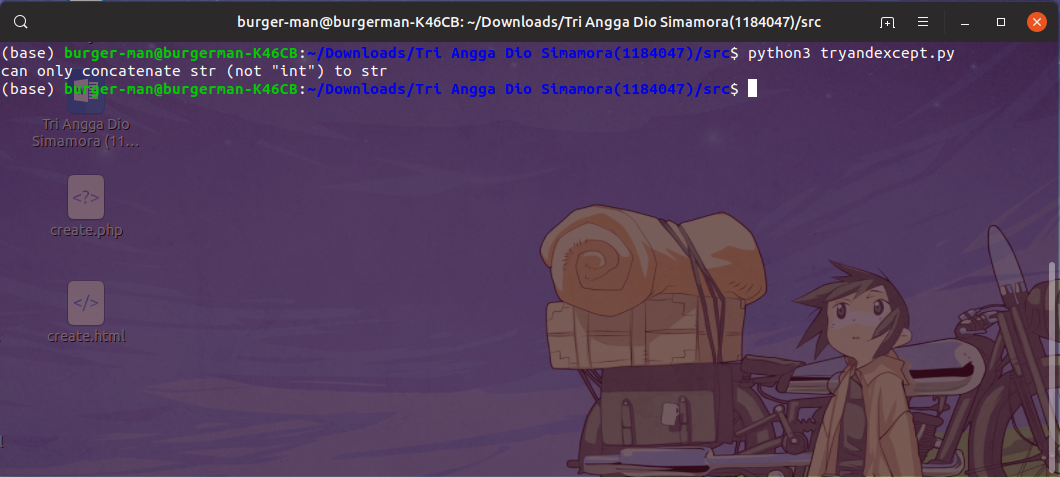
\includegraphics[width=1\textwidth]{figures/tryandexcept.png}
\caption{Gambar Try and Except}
\label{tryandexceptgbr}
\end{figure}

pada program tersebut error menjelaskan bahwa \textbf{"1"} hanya bisa di tambah oleh tipe data yang bertipe karakter juga, tidak bisa dengan integer, begitu juga sebaliknya.